\section{Bellova nerovnost}

Roku 1964 byl zveřejněn revoluční vědecký článek \parencite{bellineq}. Irský vědec John Stewart Bell tímto článkem odpověděl na myšlenkový experiment, který byl předložen Albertem Einsteinem společně s Borisem Podolskym a Nathanem Rosenem \parencite*{eprpar}. Tento myšlenkový experiment poukazuje na paradox v kvantové mechanice. Když se částice se spinem 0 rozpadne na dvě částice, podle zákonu zachování spinu musí tyto částice mít v součtu spin 0. Tomuto jevu se říká kvantové provázání. Pokud změříme spin jedné částice, instantně se dozvíme spin druhé částice, i kdyby tato částice byla vzdálena tisíce světelných let. Informace o spinu se podle kvantové mechaniky šíří mezi provázanými částicemi rychleji než světlo. Nicméně speciální teorie relativity omezuje rychlost každého kauzálního vlivu na rychlost světla. Kvantová mechanika tak porušuje lokální realismus.

Princip lokálního realismu má dvě části:
    \begin{enumerate}
        \item \textbf{Princip lokality:} objekt může být ovlivněn pouze jeho bezprostředním prostředím (Kauzální vliv se nemůže šířit rychleji než světlo). \parencite{lokalita}
        \item \textbf{Princip realismu:} vesmír existuje nezávisle na pozorovateli. \parencite{realismus}
    \end{enumerate}
    
Einstein tímto odůvodňoval svou myšlenku, že kvantová mechanika nemůže být správnou reprezentací reality. Podle něj musí každá provázaná částice nést všechny informace o svém fyzikálním stavu už od okamžiku vzniku provázání a to takovým způsobem, že jsou tyto informace nějak skryty před vlnovou funkcí kvantové mechaniky. Einstein si myslel, že musí existovat \uv{skryté proměnné}, které nejsou součástí kvantové mechaniky a spekuloval o možné teorii obsahující tyto skryté vlastnosti reality.

Bell ve svém článku \parencite*{bellineq} zveřejnil Bellovu nerovnost, pojednávající o omezení teorie se skrytými proměnnými. Aby mohla existovat teorie splňující předpoklad lokálního realismu (teorie se skrytými proměnnými) a statistické nezávislosti, musí být splněna Bellova nerovnost (viz Rovnice \ref{eq:6}, níže), podle níž musí být korelace mezi měřením propletených částic $\bm{|S|}$ menší, nebo rovna $\bm{2}$.

\begin{equation}
    \bm{|S| \leq 2}
    \label{eq:6}
\end{equation}

\clearpage

\subsection{Bellovy testy}
(Zpracováno podle článku \cite{belltest})

U jednoduchého příkladu Bellova testu (viz Obrázek \ref{fig:6}) zdroj \textbf{S} vytváří páry propletených fotonů a každý z nich vyšle v opačném směru. Oba fotony narazí na dvoukanálový polarizační filtr (\emph{a, b}), který foton odrazí, nebo propustí, podle jeho polarizace. Následně je každý foton detekován detektorem D+, nebo D- a informace o polarizaci fotonu je vyslána do korelačního monitoru CM.

\begin{figure}[ht]
    \centering
    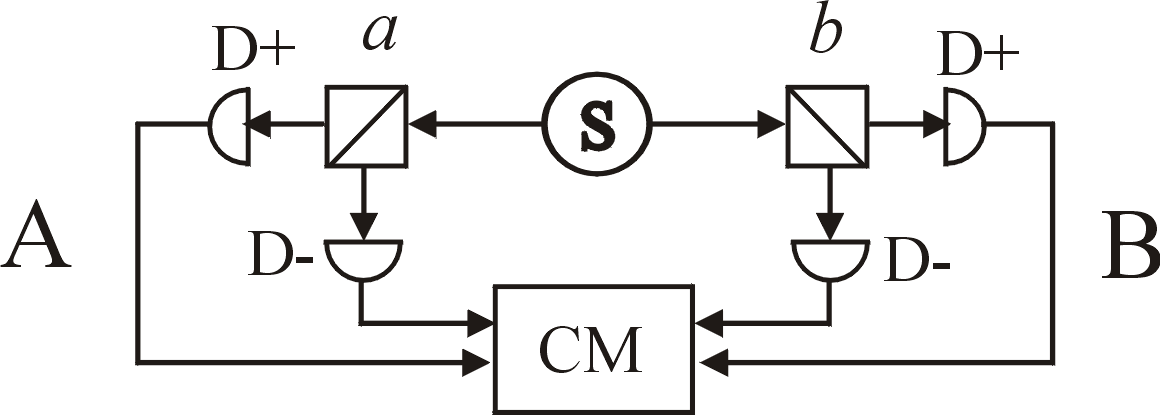
\includegraphics[width=300pt]{images/Two_channel.png}
    \caption{\label{fig:6}Schéma typického CHSH (dvoukanálového) Bellova testu.}
\end{figure}

Bell si nemohl dovolit zveřejnit článek v populárním časopise. Zveřejnil ho tedy v neznámém časopise \citejournal{bellineq}, který za příspěvky dokonce platil. Z tohoto důvodu se jeho nerovnost dočkala experimentálního pokusu až o osm let později, kdy Stuart J. Freedman a John F. Clauser změřili korelace mezi lineárními polarizacemi fotonů vyzařovaných z atomů vápníku \parencite*{belltest:1}. Korelace byla větší, než je dovoleno Bellovou nerovností. Tento výsledek byl mnohokrát replikován se stále větší přesností. Roku 2022 dostali Alain Aspect, John Clauser a Anton Zeilinger nobelovu cenu za Fyziku za experimenty s propletenými fotony, které prokázaly porušení Bellovy nerovnosti a za průkopnictví v kvantové informatice.

\subsubsection{Nepřesnosti v Bellových testech}

Nepřesnost těchto experimentů by mohla nastat z více důvodů.
\begin{enumerate}
        \item \textbf{Detekční mezera:} rozdíl mezi počtem emitovaných a detekovaných částic. 

        Garg a Mermin ukázali, že detekční účinnost ($\eta$, podíl vyslaných a změřených částic), potřebná k překonání detekční mezery u experimentu typu CHSH musí být větší než $0.83$ \parencite*{det.efficiency}. Tato hranice byla překonána roku 2001 experimentem, který dosáhl detekční účinnosti přes $0.9$ \parencite{belltest:2001}.

        \item \textbf{Mezera lokality:} možnost, že volba nastavení měření jedné částice ovlivní měření druhé částice.

        Lokalita je jedním z předpokladů potřebných k odvození Bellovy nerovnosti. Původem tohoto předpokladu je teorie relativity, která omezuje rychlost komunikace na rychlost světla. K uplatnění tohoto předpokladu u experimentu musí být doba, která uplyne mezi volbou nastavení měření\footnote[3]{Volba nastavení detektorů. V použitém příkladu (viz Obrázek \ref{fig:6}) je to volba natočení dvoukanálových polarizačních filtrů \emph{a} a \emph{b}.} a měřením samotným, kratší než doba, kterou by světelný signál potřeboval k překonání vzdálenosti mezi místy měření. U našeho příkladu (viz Obrázek \ref{fig:6}) by musela být doba mezi volbou úhlu natočení dvoukanálových polarizačních filtrů a měřením kratší, než doba, kterou by světelný signál potřeboval k cestě mezi detektory na straně A a detektory na straně B. Takový experiment navrhoval Bell už ve svém originálním článku \parencite*{bellineq}. V prvním takovém experimentu \parencite{belltest:2} byla volba nastavení měření na každé straně provedena během letu fotonů ze zdroje.

        \item \textbf{Mezera spoluvýskytu:} možnost, že zdánlivý pár propletených částic jsou doopravdy dvě částice z odlišných párů vyslaných zdrojem.
        
        U všech Bellových experimentů, zejména u experimentů založených na polarizaci fotonů, se dvojice změřených částic v obou křídlech experimentu identifikují jako patřící do jedné dvojice až po provedení experimentu, posouzením, jestli jsou jejich časy detekce dostatečně blízko sebe. To vytváří novou možnost pro lokální teorii skrytých proměnných \uv{falšovat} kvantové korelace: zpozdit čas detekce každé ze dvou částic o větší či menší množství v závislosti na určitém vztahu mezi skrytými proměnnými v částicích a nastavením detektoru, s nímž se setkají.

        Mezeře spoluvýskytu lze předejít experimentem s předem pevně danou mřížkou detekčních oken, která jsou dostatečně krátká, aby většina párů částic změřených ve stejném okně skutečně pocházela ze stejné emise, a dostatečně dlouhá, aby skutečný pár částic nebyl oddělen hranicí okna.

        \item \textbf{Paměťová mezera:} lokální teorie skrytých proměnných by mohla využít paměť předešlých nastavení měření a výsledků měření ke zvýšení porušení Bellovy nerovnosti.
        
        Bylo prokázáno, že při provedení experimentu typu Alaina Aspecta \parencite*{belltest:2} s randomizací nastavení měření nemá tato mezera dostatečný účinek ke změně výsledku experimentu \parencite{measloop:1}\parencite{measloop:2}\parencite{measloop:3}.

        \item \textbf{Superdeterminismus:} možnost porušení Statistické Nezávislosti\footnote[4]{Možnost korelace skrytých proměnných s nastavením měření.}.
        
        Tato možnost byla eliminována pod doměnkou, že by narušila \uv{svobodnou vůli} experimentátora, a že tato \uv{svobodná vůle} je nezbytná pro vědu. V následujících kapitolách zvážíme tuto možnost a ukážeme si, proč bychom jí neměli tak rychle zavrhovat.
    \end{enumerate}
    